\documentclass{article}

\usepackage[utf8]{inputenc}
% Use nameref to cite supporting information files (see Supporting Information section for more info)
\usepackage{nameref,hyperref}
% amsmath and amssymb packages, useful for mathematical formulas and symbols
\usepackage{amsmath,amssymb}
% useful for consistent display and control of units of measurement
\usepackage{siunitx}
% figures!
\usepackage{graphicx}
% for including TODO notes
\usepackage{todonotes}
% snyntax highlighting for code
\usepackage{minted}
% manually set margins
\usepackage{geometry}[margins=1in]

\title{Analysis of Equivalent Fall Height of Terrain Park Jumps: Lessons from
  Case Studies}
\author{Bryn Cloud, Mont Hubbard, Christopher Brown, Jason K. Moore}
\date{\today}

\begin{document}

\maketitle

\begin{abstract}
  Terrain parks now exist in almost all US snow sport resorts. For several decades,
  epidemiological evidence has mounted that shows increases in injuries are
  correlated with the growth in terrain park numbers. We discuss two case studies
  as evidence that large equivalent fall heights play significant roles
  in traumatic injuries at these terrain park jumps. Due to a resistant skiing industry, even with the accumulating evidence, little has been done to make jumps safer by design and deliberate clouding of the scientific truths. To help remedy
  this, we provide an accessible online tool for terrain park builders to
  both evaluate the safety of existing jumps by calculating their impact danger and to design jump shapes that control
  their impact danger. With the tools available, the barriers to designing safer
  jumps is further lowered for the ski industry to make steps in addressing the
  epidemic.
\end{abstract}

\section{Introduction}
%
When a person impacts a surface in the event of a fall, there is a risk of
injury. Greater impact velocity normal to the surface will cause greater
injury, due to the increased energy that must be dissipated. A common surrogate
for measuring impact velocity is ``equivalent fall height''.  Equivalent fall
height provides a conceptually simple and familiar interpretation of the danger
from a worse cast impact. Equivalent fall height is used in a variety of safety
standards around the world from skydiving~\todo{add citation} to children's
playground equipment~\cite{Chalmers1996}. The equivalent fall height of ski and
snowboard terrain park jumps can be calculated if the Cartesian coordinates of
the surface profile along the jumper's path and takeoff angle are
available~\cite{Hubbard2012}. Minimizing the equivalent fall height is one of
the primary jump design factors that can reduce injury. Equivalent fall height
can be controlled for and it is an obvious safety design factor to minimize
without loss of enjoyment from ski and snowboard participants.

This paper reiterates the societal cost of the increasing terrain park injuries
and then focuses on specific case studies that highlight the danger incurred if
equivalent fall height is not controlled for. We then present a user-friendly
web application for calculating equivalent fall height of existing or planned
jumps. We see this application as a part of the solution in reducing injuries
that ski jump builders can use increasing the safety in their resorts.

\subsection{History}
%
\todo[inline]{Mont should write this section.}
Terrain parks are a relatively new addition to snowsports resorts. The increase
is tied to growth in interest in aerial maneuvers and the growth of
participation in extreme sports. Unfortunately, this is correlated to an
increase injuries.  Jackson et al.~\cite{Jackson2004} determined that snow
skiing in 2004 replaced football as the second leading cause of serious head
and spinal cord injuries in the United States. It is estimated that around 10\%
of <15 year old ski and snowboard injuries are severe~\cite{Polites2018}.

\section{Equivalent Fall Height}
%
\emph{Equivalent fall height} is a commonly used as proxy measure for impact
danger by industry in safety standards~\cite{Hubbard2012}. It represents the
required kinetic energy dissipated on impact from a given height. On the
earth's surface this energy is given by the well known equation $mgh$. This is
the energy available to injure on impact in a non-rotating fall. The ability of
this energy to injure can be reduced by controlling the impact circumstances,
e.g. impact cushioning, body orientation, body configuration and active body
motion, but the energy must nevertheless be dissipated. Larger equivalent fall
heights require more intricate protection measures to reduce injury.

Equivalent fall height is a particularly useful measure of danger due to its
interpretability by lay people. People have a intuitive danger sense when faced
with potential falls from large heights and they have strong common sense for
relating fall height to likelihood of injury due to experience with falls and
observation of others' falls. For example, we have a sense of the danger
associated from falling from building stories of increasing magnitude. Ground
floor falls are on the order of 2.6~\si{\meter}, second story are
5.1~\si{\meter}, third story 8.8~\si{\meter}, and so on~\cite{Vish2005}. OSHA
requires fall protection for fall heights greater than 1.2~\si{\meter} for
general workplace safety~\todo{need citation} and the FAA's safety regulations
for safe parachuting landings is a 3~\si{\meter} fall height~\todo{need
citation}.  Chalmers et al.~\cite{Chalmers1996} pushes for 1.5~\si{\meter}
maximum fall heights for playground equipment. As for skiing, the standards for
the Olympic ski jumping call for equivalent fall heights of
0.46~\si{\meter}~\todo{need citation}.

The equivalent fall height $h$ of an object is formally defined as
%
\begin{align}
  h = \frac{v^2}{2g}
  \label{eq:efh_general}
\end{align}
%
where $v$ is the impact velocity of the object and $g$ is the acceleration due
to gravity. This definition results from equating the kinetic energy of an
object moving at velocity $v$ at impact with the potential energy of the same
object at a height $h$ above the ground.

Using Equation~\ref{eq:efh_general} as a starting point, the equivalent fall
height $h$ can be determined for any landing surface one impacts after a jump
flight trajectory~\cite{Hubbard2012}. The resulting equation, when neglecting
air drag, is
%
\begin{align}
  h = \left[\frac{x^2}{4(x\tan\theta_T - y)\cos^{2}\theta_T} -
    y\right]\sin^{2}\left[\tan^{-1}\left(\frac{2y}{x}- \tan\theta_T\right) - \tan^{-1}\frac{dy}{dx}\right]
  \label{eq:efh}
\end{align}

This equation is only a function of four variables: takeoff angle $\theta_T$,
impact coordinates $(x,y)$ on the landing surface, and the slope of the landing
surface $\frac{dy}{dx}$. It is important to note that this surface is not a
function of takeoff speed. To analyze a jump, it is sufficient to measure the
Cartesian coordinates of the landing surface along the jumper's flight path and
the takeoff angle. The slope $\frac{dy}{dx}$ can be computed from the measured
coordinates $(x,y)$.

\section{Case Studies}
%
Below we present two case studies derived from court proceedings in the United
States of America in which the jury ruled in favor of the injured plaintiffs,
in that there was neglect in the design and construction of the jumps that
contributed significantly to the injury severity of the jumpers. The results
below assume a skier mass, frontal area, and drag coefficient of 75~\si{\kg},
0.34~\si{\meter\squared}, and drag coefficient of 0.821, respectively.

\subsection{Charlene Vine v Bear Valley Ski Company}
%
In April of 2000, Ms. Charlene Vine's spine was broken when she crashed on a
jump constructed at the Bear Valley Ski Resort in California, USA. The jump
shape was that of a ``tabletop'' which is a common shape of terrain park jumps.
It is the jump constructor's intent that jumpers fully clear the table; landing
on the so called ``sweet spot'' when jumping, but Ms.~Vine landed short of the
end of the table.
Compounding the danger of a short landing, this jump's tabletop, which
would typically be flat and level, was concave.
At the 11~\si{\meter} horizontal landing distance from the takeoff point the surface
was sloped upwards approximately 5~\si{\degree}.
The upper panel of Figure~\ref{fig:vine-v-bear-valley} shows a reasonable
approximation of the jump (in black) at Bear Valley Ski Resort based on
measurements taken of the jump for the trial.
The shape of this surface highlights the detrimental effect of misaligning the
surface tangent with the jumper's flight path at impact.
%
\begin{figure}
  \centering
  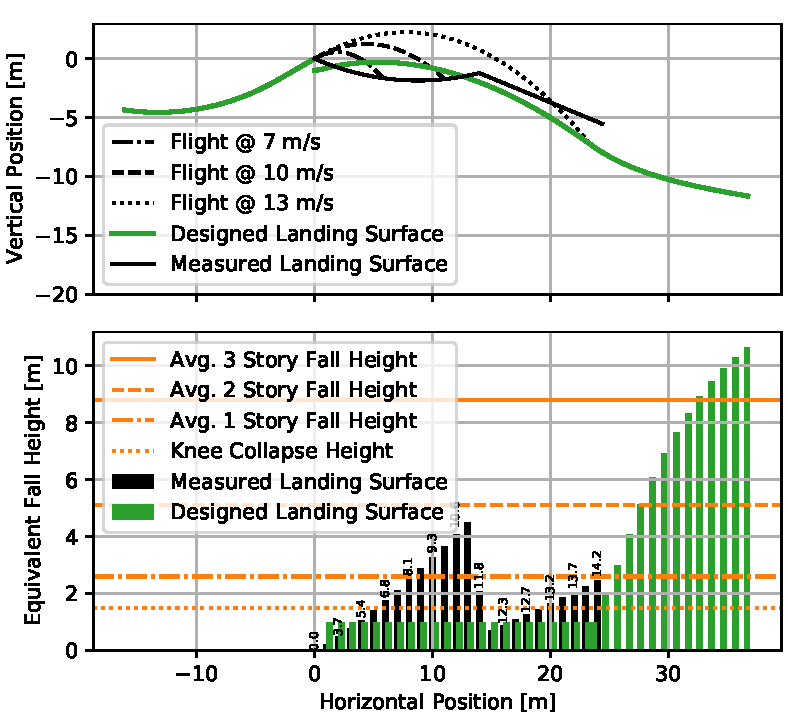
\includegraphics[width=5.25in]{figures/vine-v-bear-valley.pdf}
  \caption{\textbf{Measured Bear Valley ski jump compared to a possible design}
  The upper panel shows the cross section of the measured landing surface in as
  a solid black line. Example flight paths are shown with dashed and dotted
  black lines from the 30~\si{\degree} takeoff angle. The
  13~\si{\meter\per\second} takeoff speed is used as the design speed for a
  jump designed with constant equivalent fall height in solid green for
  comparison. The lower panel shows the equivalent fall height for both jumps
  in corresponding colors at 1~\si{\meter} intervals. The numbers above the
  black vertical bars indicate the takeoff speed in meters per second required
  to land at that location. Orange lines indicate relatable fall heights.}
  \label{fig:vine-v-bear-valley}
\end{figure}

The lower panel plots the equivalent fall height for different landing
locations on the Bear Valley jump. It is clear that short of the knuckle, the
equivalent fall height is its highest. At 11 meters, Ms.~Vine's fall height was
about 4 meters, which is equivalent to falling from between one or two storys.
The average fall heights for 1 and 2 story falls shown are estimated from data
presented in \cite{Vish2005}. ~\todo{Was her body rotated due to the concavity of the jump? Might want to add that here if so -Bryn} Ms.~Vine's body had also rotated, such that she
landed on her upper spine and was paralyzed as a result of the nearly two
story fall. The larger the equivalent fall height, the larger the impact
forces. A lower equivalent fall height would have decreased the possibility of
spinal injury, due to the lower impact forces.

On this jump, if the jumper's landing position is less than 5~\si{\meter} or
greater than 18~\si{\meter} ~\todo{Greater than 18m from where? the takeoff point? -Bryn} the equivalent fall height is less than that which
causes knee collapse~\cite{Minetti1998}, but in the range that jumpers are more
likely to land the equivalent fall height can become quite dangerous,
especially if the jumper rotates for a fall on their head as Ms.~Vine did. If a
jumper lands in the area at the end of the concave tabletop, it is equivalent
to falling out of a second story window. In contrast, a landing surface
designed to have a constant equivalent fall height can be created with a
similar amount of construction costs that would could reduce the fall height.

The green jump profile in the upper panel of
Figure~\ref{fig:vine-v-bear-valley} shows a possible jump design, derived from
a 13 m/s design speed~\cite{Levy2015}, of similar size with similar possible
flight times that ensures a constant equivalent fall height of 1~\si{\meter}.
The convex shape of this jump is interestingly close to what one would get if
the original tabletop were inverted, showing how the convex nature of the jump
shape is critically important to control equivalent fall height. A jump of this
design would have lowered impact forces for any orientation landing at any
possible landing location. In 2002, the jury ruled in favor of Ms.~Vine,
agreeing that Bear Valley was responsible for designing safer
jumps~\cite{Alvarado2002}.

\subsection{Kenneth Salvini v Ski Lifts Inc.}
%
In 2004, Kenneth Salvini attempted a table top jump with skis in the terrain
park of the The Summit at Snoqualmie ski resort in Snoqalmie, Washington, USA.
In this case, Mr.~Salvini overshot the location the jump builders' intended
landing location even while traveling at expected skiing speeds. Mr.~Salvini
somersaulted during flight and landed on his back, ultimately causing
quadriplegia. At his landing location the equivalent fall height was over 10
meters, approximately a 4 story fall height.
Figure~\ref{fig:salvini-v-snoqualmie} shows the reconstruction of the jump
profile in a solid black line based on measurements in the court proceedings.
For takeoff speeds greater than 13~\si{\meter\per\second}
(47~\si{\kilo\meter\per\hour}), the lower panel shows, also in black, that the
equivalent fall height is greater than 8 meters and grows linear with larger
takeoff speeds. Severe injury is almost certain from falls this high,
especially so if landing in a way that causes undue forces to the spine, as in
Mr.~Salvini's case.

The green curve in the upper panel is the profile of a jump designed with a
1~\si{\meter} equivalent fall height for maximum speeds of
17~\si{\meter\per\second}. This profile requires significantly more snow than
the measured jump but alleviates the dangerous impacts possible in the measured
jump.

This jump highlights how extreme the equivalent fall height can be if the jump
is not designed. Few recreational skiers will jump out of a four story window,
snow landing or not. The likelihood of injury is quite clear and our internal
altimeter.
%
\begin{figure}
  \centering
  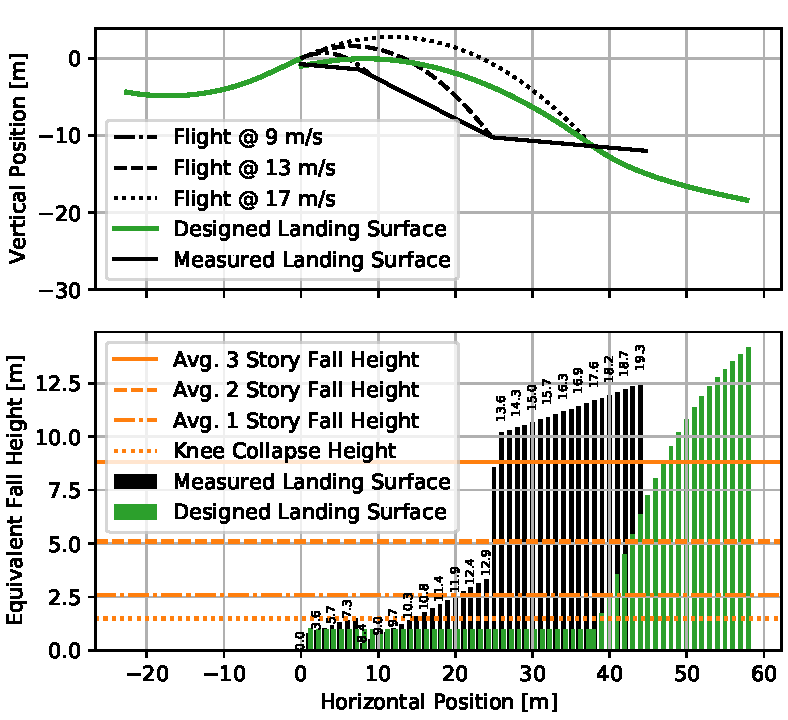
\includegraphics[width=5.25in]{figures/salvini-v-snoqualmie.pdf}
  \caption{\textbf{Measured Snoqualmie ski jump compared to a possible design}
  The upper panel shows the cross section of the measured landing surface in as
  a solid black line. Example flight paths are shown with dashed and dotted
  black lines from the 25~\si{\degree} takeoff angle. The
  17~\si{\meter\per\second} takeoff speed is used as the design speed for a
  jump designed with constant equivalent fall height in solid green for
  comparison. The lower panel shows the equivalent fall height for both jumps
  in corresponding colors at 1~\si{\meter} intervals. The numbers above the
  black vertical bars indicate the takeoff speed in meters per second required
  to land at that location. Orange lines indicate relatable fall heights.}
  \label{fig:salvini-v-snoqualmie}
\end{figure}


\section{Moral Imperative}
%
Reducing the risk of injury on manufactured terrain park jumps motivates this
work. Intelligent, engineering design based on the laws of mechanics can shape
features to limit equivalent fall height. Utilizing this fact, complies with
the first canon of engineering ethics: ``Hold paramount the safety, health and
welfare of the public''~\cite{NSPE2019}. In the context of snow sport safety,
the first canon compels engineers to direct their technical expertise to
protecting snow sport participants from injuries. None would rationally argue
that reducing equivalent fall height causes an increased likelihood of
injury and if shaping designed jump landing surfaces is no more laborious than
shaping non-designed surfaces, there are zero reasons not to attempt to control
for equivalent fall height.

People unfamiliar with the legal and insurance systems in the United States of
America might fail to appreciate that technical literature is corrupted in the
defense of unsafe practices and corporate profits. Peer-reviewed, technical
literature provides support for testimony in U.S. lawsuits. Plaintiffs and
defendants both hire their own experts to testify. Authors of technical papers
can make money by testifying. When it is for the defense, this testimony can
result in denying compensation to injuries, and serves to prolong unsafe
practices in snowsports. Rarely do experts report any conflicts of interest in
their papers and presentations, or when they organize and chair meetings or
edit publications. Financial support for publications used by expert witnesses
can be routed through consulting companies to pretend some deniability of
conflicts in their papers.

Designing jumps to limit equivalent fall height and reduce the risk of injuries
is based on well-known and well-established physics. The concept that designing
jumps to limit equivalent fall height and controlling for energy dissipation
can reduce the risk is irrefutable. Or another way to put it: impact energy in
a jump landing can be set to that of walking which has a magnitude evolution
``chose'' to guarantee the walker no injury. To counter this solid,
fundamental, scientific concept for defense experts, confounding factors are
introduced. These serve to cloud and confuse the basic issues. Consider three
examples of papers co-authored by well-known defense experts who testify for
the ski industry in ski injury cases.

Shealy et. al~\cite{Shealy2010} conducted an experimental study which attempts
to test the hypothesis that takeoff speed is a predictor of jump landing
distance. They indicate that a series of jumpers who use a terrain park jump
land within a narrow region, which is reasonable once it is noted that the
jumpers' takeoff speeds did not vary much either, i.e. no care to assess a
large range of the independent variable was taken. The authors state both that
there is ``no statistically significant relationship between takeoff speed and
the distance traveled'' and that ``takeoff speed is not a dominant or
controlling factor (in how for a jumper travels)''. These results should lead
the careful researcher to question their experimental design and analysis
methods, just as a high school physics student should if their ball does not
fall with an acceleration close to 9.8~\si{\meter\per\second\squared}.

Shealy et. al~\cite{Shealy2015} claim total serious injury rates appear not to
have changed while terrain parks increased. \todo{Read this paper and
verify/expand the claim}

In an article on landing positions~\cite{Scher2015}, Scher et. al show that
body orientation at impact can cause dangerous cervical spine loads.  They also
only test equivalent fall heights from \SIrange{0.23}{1.52}{\meter}, both
committing a similar fault as done in \cite{Shealy2010} and not testing fall
heights that are known to have caused sever injury, and yet the authors purport
that equivalent fall height has no appreciable effect on injury.

The first two studies, do a poor job of isolating variables, and were not
intended to, and the third suffers from restriction of equivalent fall height
range. But most importantly, and quite noticeably, none of these papers are
written with the intent to reduce injury rates. No ways are suggested in which
their findings could be used to promote the safety, health, and welfare of the
public. What these papers have done, is attempt to muddy the waters around the
fact that impacting a surface at a lower velocity is safer. The title of the
third paper, ``Terrain Park Jump Design: Would Limiting Equivalent Fall Height
Reduce Spinal Injuries?'' implies that the authors may believe falling on ones
head from greater and greater heights may \emph{not} cause greater injuries. It
is not clear why one might propose such a hypothesis in the first place.

Testifying for an injured plaintiff, or to defend corporations, in injury
cases, are not equivalent actions ethically, neither is authoring papers with
no intent on improving safety and reducing injuries. The former attempts to
address in problems that cause injuries, holding paramount the safety health
and welfare of the public. The latter attempts to defend the practices that
might have contributed to the injury to limit financial losses of insurance
companies. Proverbial two sides to every question do not exist in science and
engineering.

Poorly executed experiments in snowsports, no matter how expensive and
sophisticated the instrumentation, are not going to disprove the fundamental
laws of classical mechanics. If statistics or experimental results do seem in
conflict with predictions from classical mechanics, then there is a problem
with the statistical or experimental design or their interpretation, and not
with classical mechanics. Defending practices that lead to injuries at the
service of industry can prolong these practices, which can lead to further
injuries, clearly violating the first canon of engineering ethics.

\section{What Can Be Done?}
%
Assessing and reshaping existing jumps for dangerous equivalent fall heights is
a very low hanging opportunity for ski resorts to reduce the danger of their
terrain park jumps. Accurate enough measurements of an existing slope can be
done with simple tools, e.g. a tape measure and a digital level, and only takes
a short amount of time per jump, see Appendix~\ref{sec:jump-shape-measurement}.
The calculation and visualization of the equivalent fall height from these
measurements can take some time if manually done but we are are making
available an online, freely accessible, and user friendly web application that
makes the calculation and visualization step almost instantaneous for the
terrain park builder. With the tool described in the next section, terrain park
builders can easily add this safety assessment to their toolbox, even using it
from a smartphone while in the field. There is no reason that this basic
assessment should not be part of the jump construction process. The laws of
nature clearly tell us that designing jumps with lower equivalent fall heights
will have a positive probability in reducing injuries.  The only ethical
decision is to adopt these methods as saving even one person from a life of
paralysis must be worth the minor inconvenience of shaping jumps using these
rules in \cite{Levy2015}.

\subsection{Software and Online Access}
%
Previously, we developed software for designing ski jumps with a constant
equivalent fall height~\cite{Moore2018}. The software comprises of a general
purpose, extensible, object oriented software library with tools for 2D skiing
simulation. Using the library code, a web application was developed for
interactive jump design. The web application is designed for a non-technical
end user and usable on a desktop, tablet, or mobile device; any device that
supports a web browser.

We have extended the capabilities of the software in version 0.2.0 for the
purposes of the work described in this paper. New library features were added
that automate the calculation of equivalent fall height for jump profiles
described by a series of Cartesian coordinates.
Additionally, a new
``analysis'' page was added to the web application which allows users to upload
either a comma separated value CSV text file or a Microsoft Excel spreadsheet
file or with the jump profile coordinates. The jump is then analyzed and the
equivalent fall height is displayed graphically for interactive user
manipulation and viewing. Figure~\ref{fig:web-app-screenshot} shows the web
application with one of the case study jumps loaded for analysis.
%
\begin{figure}
  \centering
  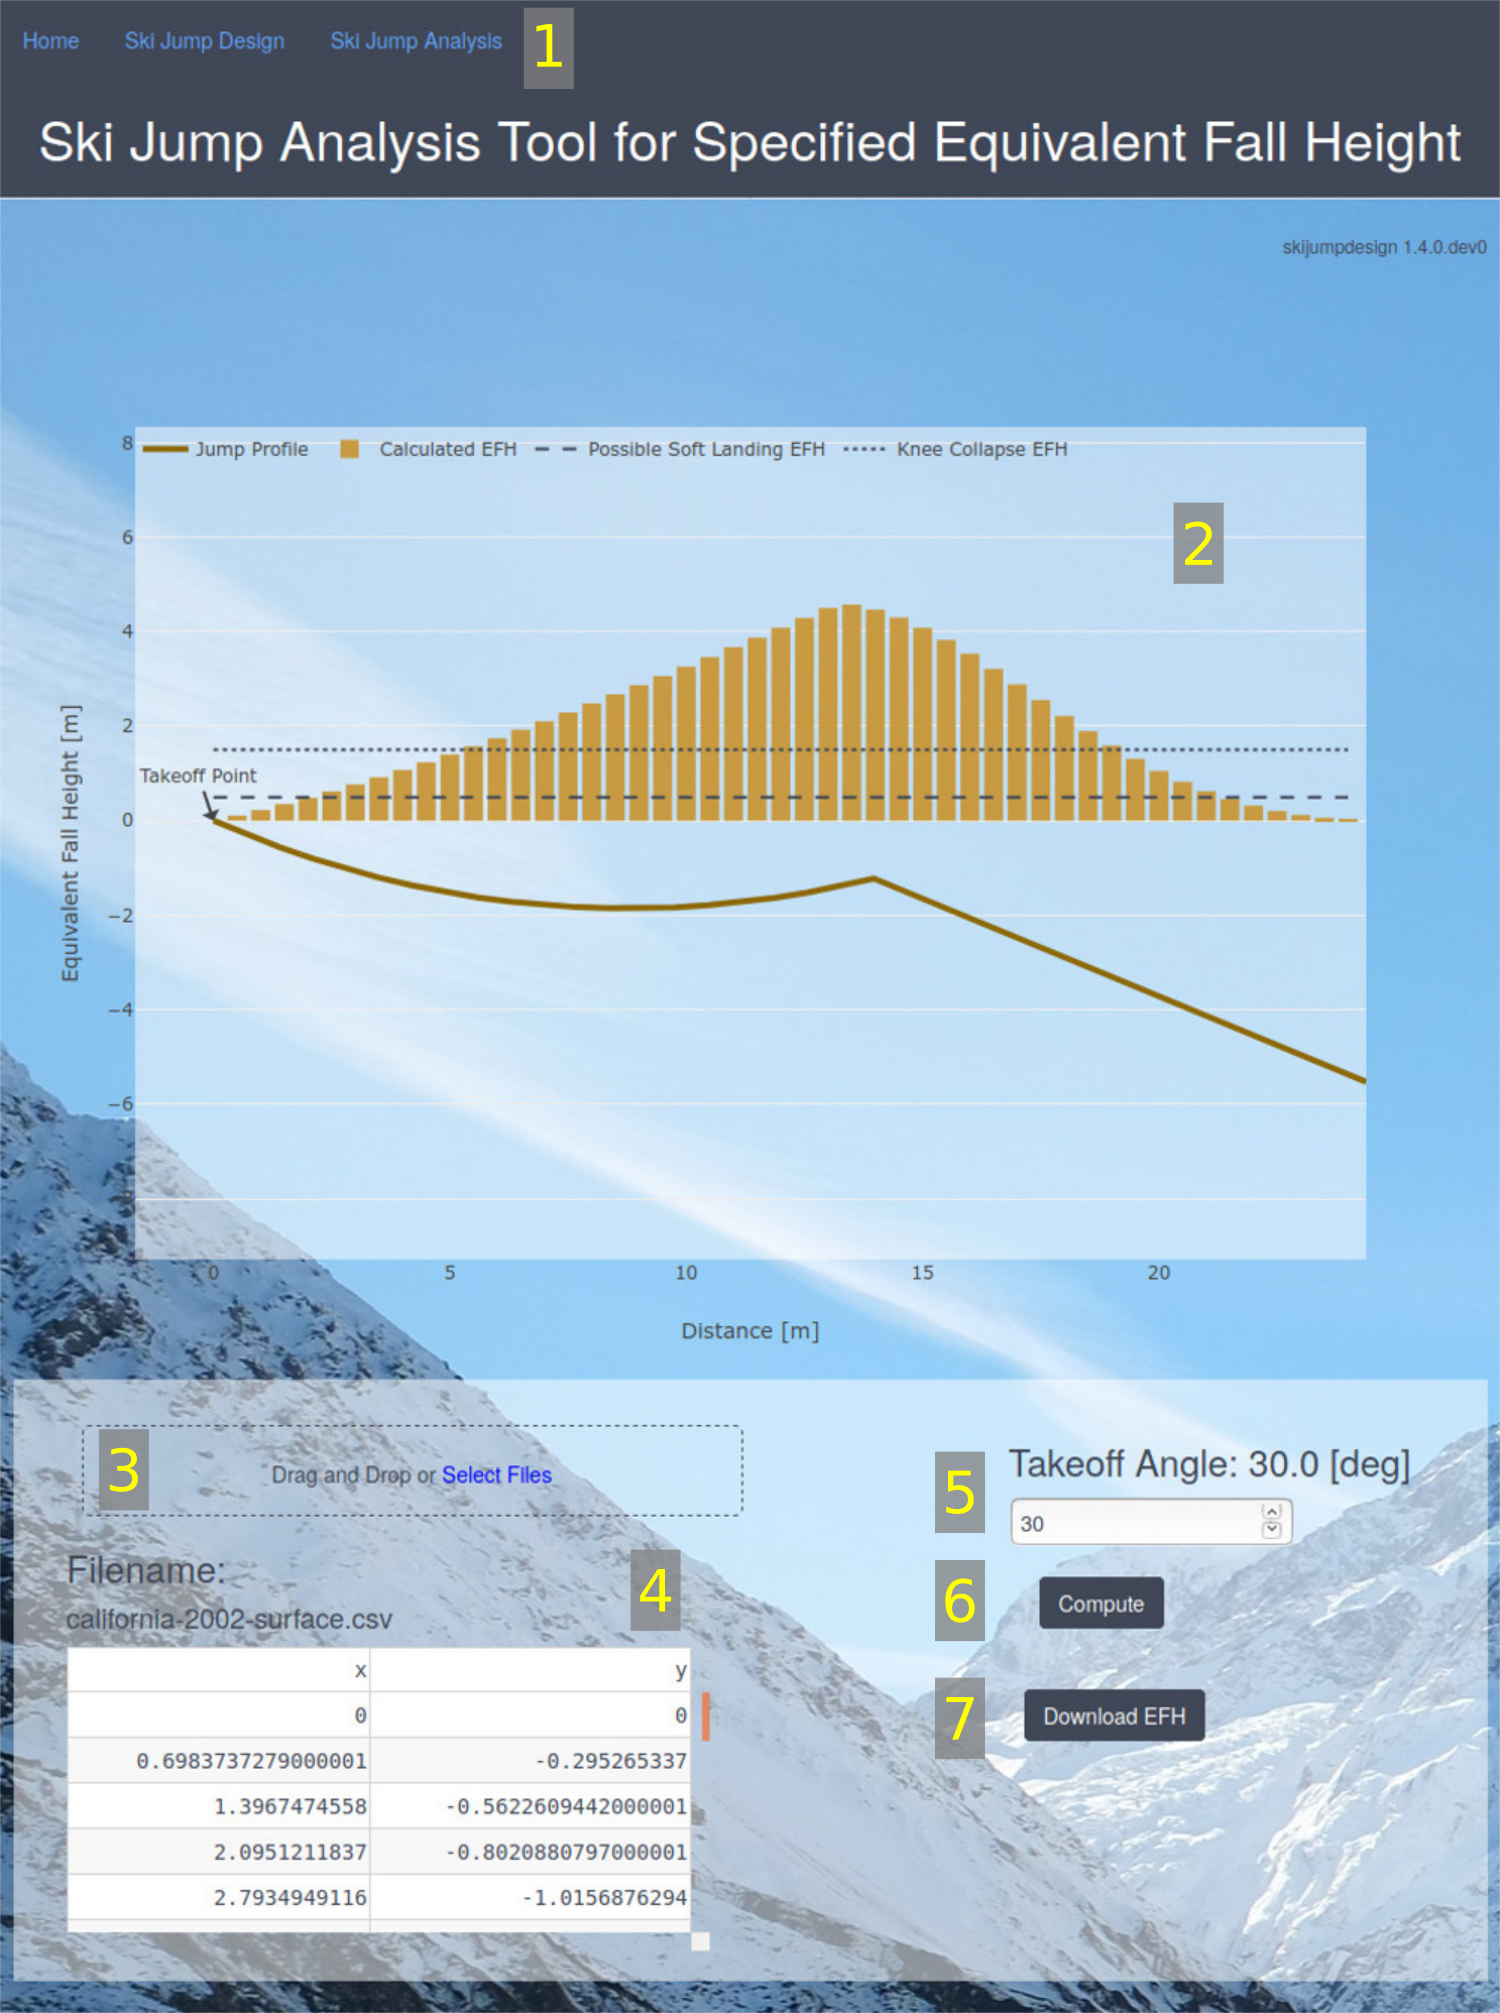
\includegraphics[width=5.00in]{figures/web-app-screenshot.png}
  \caption{\textbf{Screenshot of the web app} To use the app, a user selects
    ``Ski Jump Analysis'' from the primary menu [1], uploads a CSV or XLS file
    by dragging it onto the screen [3], inspects the input data for accuracy in
    the table [4], sets the takeoff angle [5], runs the analysis by pressing
    the ``Compute'' button [6], views the results in the interactive plot [2],
    and downloads the results by pressing the ``Download EFH'' button [7].}
  \label{fig:web-app-screenshot}
\end{figure}

The software is written in Python and directly depends on popular packages
including Cython~\cite{Behnel2011}, matplotlib~\cite{Hunter2007},
NumPy~\cite{Oliphant2006}, pandas~\cite{McKinney2020},
Plotly/Dash~\cite{Plotly2015}, pycvodes~\cite{Dahlgren2018},
SciPy~\cite{Virtanen2020}, SymPy~\cite{Meurer2017}, and xlrd.
The software is open source and licensed under the MIT redistribution license.
The source code is available on Gitlab
(\url{https://gitlab.com/moorepants/skijumpdesign}) and PyPi
(\url{https://pypi.org/project/skijumpdesign/}. Users can submit bug reports, feature
requests, code improvements, and additions at the Gitlab repository. The
software is documented at
\href{https://skijumpdesign.readthedocs.io}{skijumpdesign.readthedocs.io}.
Basic examples of using the library are provided in the appendix.

\section{Conclusion}
%
There are, of course, more factors than jump landing surface shape that
contribute to injuries on terrain park jumps but impact velocity can be easily
controlled with a designed landing surface. There is no evidence to support
that decreasing equivalent fall height increases injuries in falls, only
evidence that injuries can be decreased. Thus there is no reason not to adopt
constant equivalent fall heights of low values for public use jump designs.
Common sense is really all that is needed to believe that falling from higher
heights will increase injury to human bodies regardless of other factors.
Constructors of terrain park jumps that are not designed with these facts in
mind are negligent. The safety, health, and welfare of the public involved in
this sport is paramount.

\bibliographystyle{unsrt}
\bibliography{references}


\appendix

\section{Example software library use}
%
This closed form equations are useful for understanding the fundamental
relationship of equivalent fall height to the landing surface and well predict
these values for small jumps but other factors may be useful to include in the
model. For example, jumpers are subject to aerodynamic drag and this is not
negligible for larger jumps. If drag is included there is no closed form
solution for the equivalent fall height, but the equivalent fall height can be
computed through iterative simulation~\cite{Levy2015}. The jumper's flight path
is found by integrating the flight equations of motion at various takeoff
velocities and computing the misalignment in jumper landing angle and the slope
angle to then find the equivalent fall height. This more general simulation
method is implemented in the software described herein and the results reflect
the inclusion of gravitational and drag forces. The simulations require
measurements of the landing surface cross-sectional profile coordinates $(x,y)$
relative to the takeoff point and a measurement of the takeoff angle.

Listing~\ref{lis:example-efh-calc} demonstrates creating a surface from some
measured data points and then calculating the equivalent fall height at
0.2\si{\meter} increments.
%
\begin{listing*}
  \begin{minted}{pycon}

>>> import numpy as np
>>> from skijumpdesign import Surface, Skier
>>> takeoff_ang = 10  # degrees
>>> takeoff_point = (0, 0)  # meters
>>> x_ft = np.array([-232.3,-203.7,-175.0,-146.3,-117.0,-107.4,
...    -97.7,-88.0,-78.2,-68.5,-58.8,-49.1,-39.4,-34.5,-29.7,
...    -24.8,-19.8,-17.8,-15.8,-13.8,-11.8,-9.8,-7.8,-5.9,-3.9,
...    -2.0,0.0,0.0,0.0, 2.0,3.9,5.9,7.9,9.9,11.9,13.9,15.9,
...    17.9,19.9,21.9,23.9,25.8,27.8,29.7,31.5,33.4,35.2,37.0,
...    38.8,43.3,47.8,52.3,56.8,61.5,66.2,70.9,75.7,80.6,85.5,
...    88.4,88.4])
...
>>> y_ft = np.array([55.5,46.4,37.7,29.1,22.2,19.7,17.2,14.8,
...    12.5,10.2,7.7,5.2,2.9,1.8,0.7,-0.2,-1.0,-1.2,-1.4,-1.6,
...    -1.7,-1.6,-1.5,-1.3,-1.0,-0.4,0.0,0.0,0.0,-0.3,-0.8,
...    -1.0,-1.4,-1.4,-1.5,-1.5,-1.5,-1.5,-1.6,-1.8,-2.0,-2.4,
...    -2.9,-3.5,-4.2,-5.0,-5.8,-6.7,-7.5,-9.8,-12.0,-14.2,
...    -16.2,-18.1,-19.8,-21.4,-22.9,-24.0,-25.0,-25.6,-25.6])
...
>>> x_mt = x_ft*0.3048 # convert to meters
>>> y_mt = y_ft*0.3048 # convert to meters
>>> # create a surface from the data
>>> measured_surf = Surface(x_mt, y_mt)
>>> # use the default skier properties for simulations
>>> skier = Skier()
>>> # calculate the equivalent fall height
>>> x, efh = measured_surf.calculate_efh(
...     np.deg2rad(takeoff_ang), takeoff_point, skier, increment=0.2)
...
>>> x  # display the x coordinates
array([ 0. ,  0.2,  0.4,  0.6,  0.8,  1. ,  1.2,  1.4,  1.6,  1.8,  2. ,
        2.2,  2.4,  2.6,  2.8,  3. ,  3.2,  3.4,  3.6,  3.8,  4. ,  4.2,
       ...
       24.2, 24.4, 24.6, 24.8, 25. , 25.2, 25.4, 25.6, 25.8, 26. , 26.2,
       26.4, 26.6, 26.8])
>>> efh  # display the equivalent fall height for each x coordinate
array([0.        , 0.02541035, 0.03479384, 0.03264587, 0.05956476,
       0.09096091, 0.12358184, 0.13702364, 0.15202999, 0.17018343,
       ...
       3.93910556, 3.97387212, 4.00891899, 4.04424779, 4.07984952,
       4.11573359, 4.68049185, 5.53413479, 6.45253722, 7.42628019])
  \end{minted}
  \caption{Python interpreter session showing how one could compute the
  equivalent fall height of a measured jump.}
  \label{lis:example-efh-calc}
\end{listing*}

\section{Jump Shape Measurement}
\label{sec:jump-shape-measurement}
%
Equation~\ref{eq:efh} requires the Cartesian coordinates and slope of the
landing surface along the path of the jumper. There are a number of possible
measurement techniques for collecting data adequate for the equivalent fall
height calculation but the simplest method only requires a digital level
\footnote{smartphone level measurement applications are likely sufficient and
readily available}, a flexible tape measure, and less than an hour's time from
one person per jump. A tenth of a degree accuracy from the level and down to 25
centimeter accuracy from the tape measure should be sufficient for typical snow
sport jumps varying jumps.

To measure the jump, the takeoff point should be identified and the tape
measure should then be draped over the contour of the landing surface along the
projection of the expected flight path onto the landing surface. The origin of
the tape measure should be aligned with the takeoff point. Starting with the
takeoff point, the digital level should be used to record the absolute angle at
regular increments along the tape. The increment can be varied between
25~\si{\centi\meter} and 100~\si{\centi\meter}, with the former used for steep
slope changes and the later for less steep; 50~\si{\centi\meter} increments are
appropriate for average jump shapes. Positive angles should be recorded for
positive slope and negative angles for negative slope. The tabulated data
should include the distance along the surface from the takeoff point, $d_i$,
and the associated surface angle, $\theta_i$, at each distance measurement for
$n$ measurements. Assuming $\theta_i$ is in radians, the Cartesian coordinates
can be computed using the average angle to find the adjacent coordinates. The
following equations show provide the necessary data for the calculation of
equivalent fall height:
%
\begin{align}
  \frac{dy}{dx}_{i} & = \arctan{\theta_i} \\
  x_{i + 1} & =
  \begin{cases}
    0 & \text{for } i=0 \\
    x_i + (d_{i+1} - d_i)\cos{(\theta_{i+1} + \theta_i)/2} &  \text{for } i=1\ldots n
  \end{cases} \\
  y_{i + 1} & =
  \begin{cases}
    0 & \text{for } i=0 \\
    y_i + (d_{i+1} - d_i)\sin{(\theta_{i+1} + \theta_i)/2} &  \text{for } i=1\ldots n
  \end{cases}
\end{align}

Listing~\ref{lis:example-meas-calc} demonstrates calculating the landing
surface's Cartesian coordinates from measured distance and angle data collected
with the method described above.
%
\begin{listing*}
  \begin{minted}{pycon}
>>> from skijump.functions import cartesian_from_measurements
>>> dis = [14.5, 15.0, 15.5, 16.0, 16.5, 17.0]  # meters
>>> ang = np.deg2rad([4.6, -7.4, -16.5, -9.7, -11, -6.9])  # radians
>>> x, y, to_point, to_angle = cartesian_from_measurements(dis, ang)
>>> print(x)  # meters
[0.         0.49985074 0.98901508 1.47600306 1.96786738 2.46177962]
>>> print(y)  # meters
[ 0.         -0.01221609 -0.1157451  -0.22907075 -0.31890113 -0.39668737]
>>> print(to_point)  # takeoff point in meters
(0.0, 0.0)
>>> print(to_angle)  # takeoff angle in radians
0.08028514559173916
  \end{minted}
  \caption{Python interpreter session showing how one could compute the
  Cartesian coordinates from equivalent fall height of a measured jump.}
  \label{lis:example-meas-calc}
\end{listing*}

\end{document}
